\documentclass[../revisedmain.tex]{subfiles}
\begin{document}
Moving onto a related topic, it can be beneficial to calculate the area underneath a graph of some function. For example, the area underneath a graph between two points $a$ and $b$ can be used to find the average value of a graph. We can't exactly find the area underneath most graphs because there are no formulas for the area of an area bounded by, say, $f(x)=2x\sin(x^2)+5$. However, we can approximate the area using different methods. Four that will be covered on the AP test are:
\begin{enumerate}
	\item \textbf{Left Riemann Sum}
	\begin{center}
	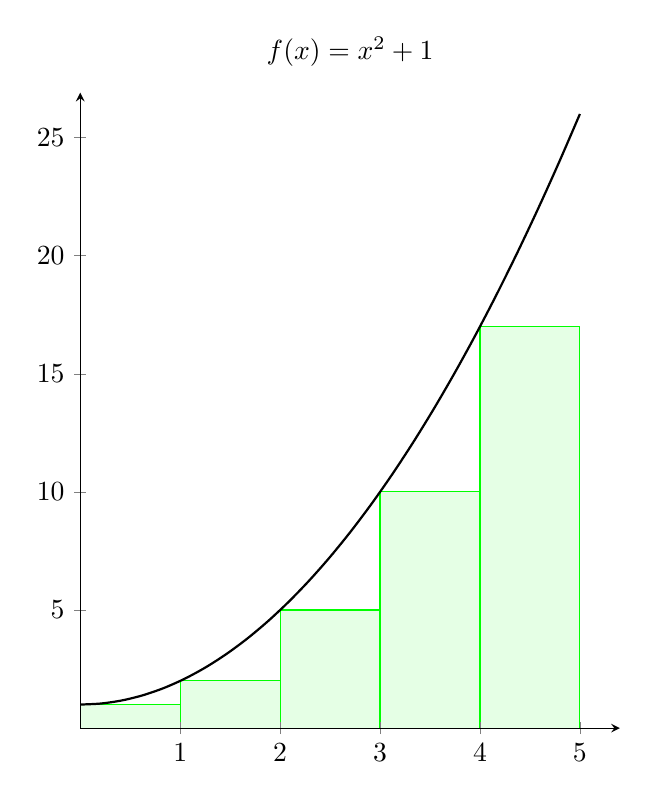
\begin{tikzpicture}
		\begin{axis}[
			xtick={0,...,5},ytick={5,10,15,20,25},
			y=0.3cm, xmax=5.4,ymax=26.9,ymin=0,xmin=0,
			enlargelimits=true,
			axis lines=middle,
			clip=false,
			domain=0:5,
			axis on top,
			title={$f(x)=x^2+1$}
			]
			\addplot [draw=green, fill=green!10, ybar interval, samples=6]{1+x^2}\closedcycle;
			\addplot[smooth, thick,domain=0:5]{1+x^2};
		\end{axis}
	\end{tikzpicture}
	\end{center}
	The Left Riemann sum divides an interval from $a$ to $b$ into $n$ subintervals and adds together rectangles stretching up from the $x$-axis until the \textit{left} corner touches the graph. In this case, [0,5] is divided up into 5 subintervals with width 1 each. The heights for the rectangles are $f(0)$, $f(1)$, $f(2)$, $f(3)$, and $f(4)$ because they are the left endpoints. The sum of $n$ rectangles is:$$(width_1*height_1) + (width_2*height_2) + \dots +(width_n*height_n)$$ In Riemann sums, the widths are all equal, so the sum siplifies to:$$width*(height_1+height_2+\dots+height_n)$$ which in this case is:$$1*\left(f(0)+f(1)+f(2)+f(3)+f(4)\right)$$$$=1+2+5+10+17$$$$=35$$
	\item \textbf{Right Riemann Sum}
		\begin{center}
			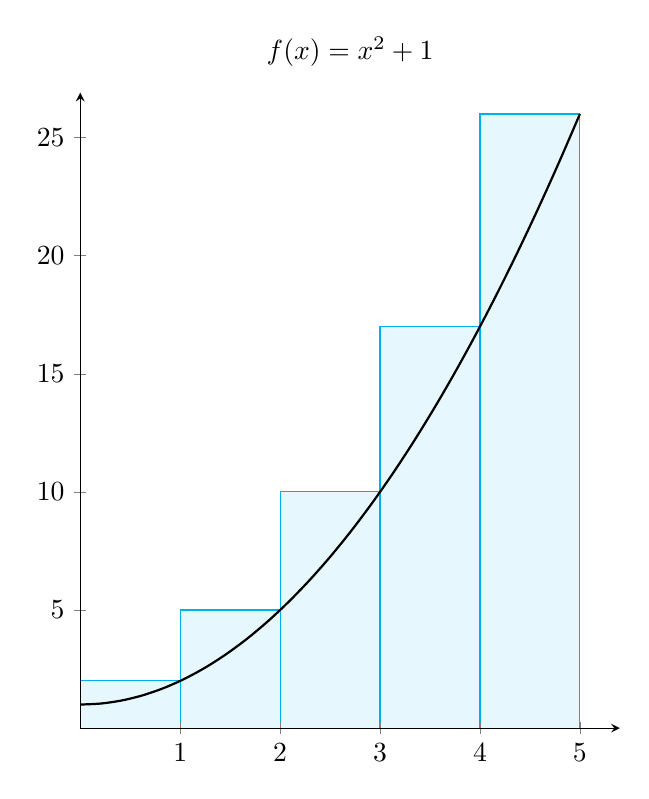
\begin{tikzpicture}
			\begin{axis}[
			xtick={0,...,5},ytick={5,10,15,20,25},
			y=0.3cm, xmax=5.4,ymax=26.9,ymin=0,xmin=0,
			enlargelimits=true,
			axis lines=middle,
			clip=false,
			domain=0:5,
			axis on top,
			title={$f(x)=x^2+1$}
			]
			\addplot [draw=cyan, fill=cyan!10, ybar interval, samples=6]{1+(x+1)^2}\closedcycle;
			\addplot[smooth, thick,domain=0:5]{1+x^2};
			\end{axis}
			\end{tikzpicture}
		\end{center}
		The Right Riemann sum is identical to the Left Riemann Sum except that it evaluates the function at the \textit{right} side. In this case, the approximation is:$$1*(f(1)+f(2)+f(3)+f(4)+f(5))$$$$=2+5+10+17+26$$$$=60$$
	\item \textbf{Midpoint Riemann Sum}
		\begin{center}
			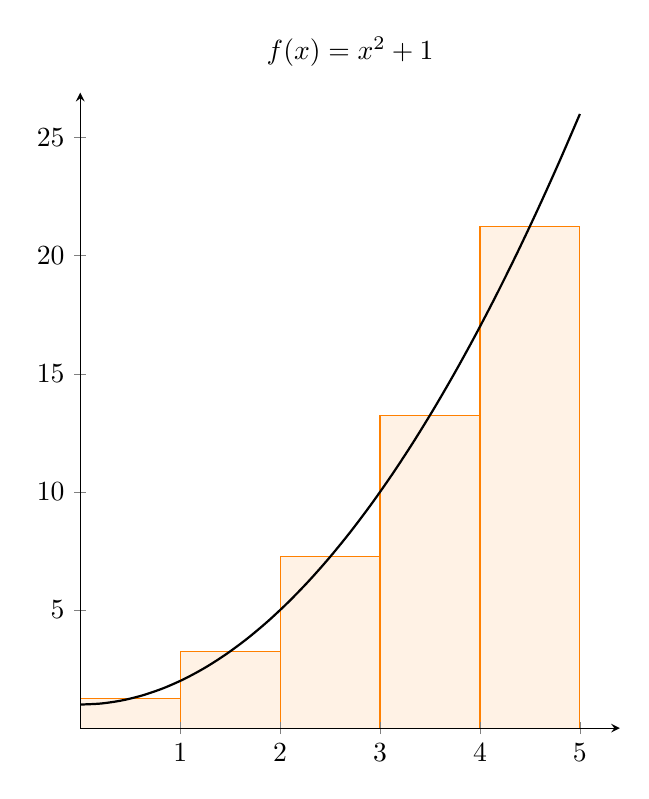
\begin{tikzpicture}
			\begin{axis}[
			xtick={0,...,5},ytick={5,10,15,20,25},
			y=0.3cm, xmax=5.4,ymax=26.9,ymin=0,xmin=0,
			enlargelimits=true,
			axis lines=middle,
			clip=false,
			domain=0:5,
			axis on top,
			title={$f(x)=x^2+1$}
			]
			\addplot [draw=orange, fill=orange!10, ybar interval, samples=6]{1+(x+.5)^2}\closedcycle;
			\addplot[smooth, thick,domain=0:5]{1+x^2};
			\end{axis}
			\end{tikzpicture}
		\end{center}
		Just like the other two, the only difference is that the Midpoint Riemann Sum calculates at the midpoint of the subintervals, so the approximation is:$$1*(f(0.5)+f(1.5)+f(2.5)+f(3.5)+f(4.5))$$$$=1.125+3.25+7.25+13.25+21.25$$$$=46.125$$		
	\item \textbf{Trapezoidal Sum}
	The trapezoid sum has the potential to have the least error of any of the previous 3 methods. Instead of summing rectangles, it sums trapezoids that look identical to the rectangles but instead of being a rectangle on the top, the top is bounded by a line that starts at $(a,f(a))$ and ends at $(b,f(b))$ instead of being a horizontal line at one of those points. The area of a trapezoid is $\displaystyle\frac{h}{2} (base_1+base_2)$. In this case, the bases are vertical and the width is the total interval divided into $n$ subintervals. Therefore, the total area for one trapezoid from $x=a$ to $x=b$ would be:$$\frac{width}{2} (f(a)+f(b))$$ If we were to add up all of these rectangles over an interval [c,d] divided into $n$ subintervals, the area would be:$$\frac{\frac{d-c}{n}}{2} (f(c)+f(c+\frac{d-c}{n})+\frac{\frac{d-c}{n}}{2} (f(\frac{d-c}{n})+f(c+2\frac{d-c}{n})+\dots+\frac{\frac{d-c}{n}}{2} (f(d-\frac{d-c}{n})+f(d)$$$$=\frac{d-c}{2n}\left(f(c)+f(c+2\frac{d-c}{n})+2f(c+2\frac{d-c}{2})+\dots+2f(d-\frac{d-c}{n})+f(d)\right)$$If we were to abbreviate the width $\displaystyle\frac{d-c}{n}$ as $i$, it simplifies down to:$$\frac{i}{2}\left(f(c)+2f(c+i)+2f(c+2i)+\dots+2f(d-i)+f(d)\right)$$The trapezoid approximation is somewhat complex yet elegant at the same time.
\end{enumerate}
\end{document}